\section{讨论:从头均采食量到草料投放量}
\label{discussion}

本工作直接进行预测的目标是未来一天的头均采食量,而不是应当投喂的草料量,主要是因为草料的投放受人的主观因素影响,实际草料的投放取决于饲养员的策略。草料的投放是\emph{草料成本}和\emph{奶牛采食量}的这两者的权衡折衷。过高的投放量能保证牛吃饱,但会造成草料的浪费,提高牧场的运营成本;过低的投放量节约了成本,但会造成奶牛采食不足,影响产奶量,降低经济效益。因此饲养员希望制定适中的草料投放量。牧场规定各牛舍最佳草料投放量应使草料有剩余,但剩余控制在(草料投放量的)5\%以内。

假设存在完美的采食量预测器可以零误差地精确预测未来一天各牛棚的采食量,则问题很简单,饲养员只需要按照采食量预测值再稍加少许饲料(避免奶牛吃太多土)投放即可。但世界上不存在完美的预测器,机器学习的模型总会存在一定的预测误差。我们暂时假设在提前指定草料投放量后,饲养员不再有机会临时变更草料投放量(减草或加草)。因而完全根据预测器的输出来指定采食量会有两种风险:草料投放过多的风险和草料投放不足的风险。这两种哪种后果更严重取决于它们二者带来的经济损失:是牛没吃够导致奶产量下降的经济损失大,还是过多投放的草料成本大。一般而言,如果我们假设前者的损失更大,应当尽力避免草料投放不足,则我们会考虑在模型对采食量的预测值的基础上适当增加一定量进行投放。难点在于该增加量如何确定。

\begin{figure}
\begin{center}
	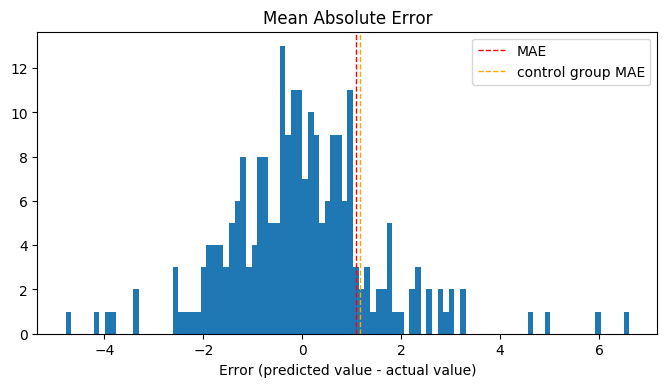
\includegraphics[width=0.95\linewidth]{error_dist}
\caption{表\ref{table_total_concat}中最优结果对应的参数配置下,某次交叉验证中测试集上误差的分布。虚线标注测试集和对照组的$\epsilon_{MAE}$。}
\label{error_dist}
\end{center}
\end{figure}

我们首先观察模型预测误差的分布。图\ref{error_dist}显示了最优结果($\epsilon_{MAE} = 1.0788$)对应的参数配置下(w=4,头均产奶量时间序列一层小波分解,max\_depth=4,n\_enumerator=100),一次交叉验证实验中,测试集各样本上的误差分布情况。观察可以发现误差分布较分散(方差较大),分布整体近似正态分布的钟形曲线,即大部分样本上误差接近0,误差越大的样本数量越小。虽然我们的模型能够有效提升头均采食量的预测精度(图中从橙色虚线1.1590降低至红色虚线1.0788),但和预测误差的标准差(1.51)相比,预测精度的提升仍然非常有限,仍存在少部分样本预测误差较大。例如,在12\%的(29/237)的样本上,预测误差的绝对值大于1.5(若采食量为30千克,多放了1.5千克的草料意味着剩料约为4.8\%),在3\%(7/237)的样本上,预测误差的绝对值甚至大于3。

如果我们只有一次制定草料投放量的机会,设我们实际投放$\hat {y_t} + \Delta$的(头均)草料($\hat {y_t}$是模型对头均采食量预测值,$\Delta$是降低牛采食不足风险的校正增量),则在误差分布图\ref{error_dist}中,所有位于直线$x_0=-\Delta$左边的样本点对应“奶牛采食不足”\footnote{或者说,钟型曲线在直线左边部分的面积占曲线下总面积的比例,是“奶牛采食不足”的概率。},而所有其他横坐标为$x > x_0 = -\Delta$的样本点对应的剩草率为$(x + \Delta) / y_t$。可见如果$\Delta$不断增大,采食不足的样本点数量会减少,但所有样本的整体剩草率会升高。因此在将本工作提出的预测模型运用到实践中时,还需要面临的挑战是如何确定合适的$\Delta$,即:实际投放的头均草料量应当比模型给出的预测值高多少。

上述问题超出本文讨论的范围,但我们对于优化剩草率这一最终目标,给出如下几点思考。

(1) 从\textbf{影响奶牛采食量的因素}和\textbf{饲养员}角度讲,模型的输入变量并未涵盖所有影响奶牛采食量的因素,这对模型的预测不可避免地带来误差。作为饲养员,对牛群的状态有更全面的了解,例如对于调群事件(以及导致调群的背后逻辑)给牛群带来的影响有更多掌握,对于疫苗注射、环境变化等对牛可能造成应激反应的情况也了解更多等等。因此饲养员不必拘泥预测器给出的采食量预测值,而是可以结合经验、当前的实际情况和模型的输出,更灵活地调节草料投放量。

(2) 从\textbf{模型的预测能力}角度讲,当前模型预测误差的精度提升有限,且误差方差大,这限制了模型在实际中发挥的作用。未来改进的方向还是通过扩充数据集,增加更多对采食量有显著影响的因素作为特征,以及改进特征的提取、变换方式,进一步降低模型预测的误差。

(3) 从\textbf{草料制备的策略}角度讲,对草料量进行一次甚至多次的反馈控制(根据已投放草料的采食情况决定是否临时增减当天的总草量)是降低采食不足和剩草过多风险的重要手段。当前牧场制备草料的时间粒度大致为1天(报草时确定未来1天的草料总量),如果有可能,可以考虑实现更精细的备料时间粒度,实施少量多次的草料制备,这样每次制备草料的量可以根据当天牛进行采食的实时情况进行动态地调整。但该思路也需要将少量多次的草料制备和多次草料运输、投放等工作的成本纳入计算。如总成本不降反升,则不值得。

(4) 从\textbf{草料投放的策略}角度讲,一个优化思路是对已投放的草料在空间上进行再平均。简单地说,就是根据各牛舍的采食情况,把剩草比较多的牛舍中一部分草料转移到某些草料即将吃完的牛舍中进行二次投放。这样互通盈余,理论上可以降低牧场的总剩草率。但是和(3)类似,该策略需要考量实际操作的相关成本,判断是否值得。







